%%%%%%%%%%%%%%%%%%%%%%%%%%%%%%%%%%%%%%%%%%%%%%%%%%%%%%%%%%%%%%%%%%%%%%%%%%%%%%%%%%%%%%%%
\section{Introduction} \label{sec_intro}
%%%%%%%%%%%%%%%%%%%%%%%%%%%%%%%%%%%%%%%%%%%%%%%%%%%%%%%%%%%%%%%%%%%%%%%%%%%%%%%%%%%%%%%%

This paper deals with a discontinuous finite element spatial discretizations of the radiation 
diffusion equation on arbitrary polygonal grids, with and without adaptive mesh refinement. 
Radiation diffusion is an asymptotic limit of the radiation transport equation and can be 
written in the following form:
\begin{equation} \label{eq:radiation_diffusion}
- \div  D(\vr) \grad E(\vr) + \sigma_a(\vr) E(\vr) = Q(\vr) ,
\end{equation}
where $E$ is the radiation energy intensity, $D$ is a diffusion coefficient, $\sigma_a$ is 
an opacity coefficient, and $Q$ is the source.

Several spatial discretizations have been proposed to solve \eqt{eq:radiation_diffusion} on
arbitrary polygons (2D) and polyhedra (3D) \cite{Wachspress,MorelDendyHallWhite1992,
PalmerLLNL,Palmer2005,MorelHallShashkov,BaileyAdams2008,KutnetsovMimetic}. 

Wachspress \cite{Wachspress} developed a family of rational polynomial functions that can be employed
as basis functions in a finite element method on polygonal/polyhedral grids. This yields
symmetric positive-definite (SPD) matrices but (i) the finite element integrals must be carried out 
numerically and (ii) the Jacobian of the transformation becomes zero on degenerate cells 
(such as the ones shown on \fig{fig:amr_schematics}). 
%
Morel et al. \cite{MorelDendyHallWhite1992} introduced a cell-centered finite volume scheme 
for arbitrary quadrilateral meshes. Their scheme was second-order accurate and yielded back a 
standard five-point stencil on orthogonal grids, but the diffusion operator was asymmetric 
and cell-edge unknowns were added in addition to cell-center unknowns.
%
Palmer \cite{PalmerLLNL,Palmer2005} proposed a node-based finite volume method 
that enforces particle balance over dual cells, where a dual cell is defined as 
the union of all corners surrounding a given vertex $p$ and where  a corner 
is a quadrilateral defined by vertex $p$, the cell center, and the midpoint
of the edges that contain vertex $p$. On a triangular grid, Palmer's scheme is equivalent 
to linear continuous finite elements with ``mass-matrix lumping''. The method is 
second-order accurate but the discretization of the diffusion equation using Palmer's method 
does not result in SPD matrices.
%
Mimetic finite difference methods create discrete analog of vector and tensor
calculus in order to accurately approximate the original differential operators;
see, e.g., \cite{HymanMorelShashkovSteinberg2002}.
Mimetic methods preserve important properties of the differential operators such 
as symmetry, positivity, monotonicity, asymptotic limits, and identities pertaining 
to tensor and vector calculus. Mimetic methods can also be viewed as mixed hybrid 
finite element formulations with specific spatial quadratures.  
Mimetic finite difference methods have been applied to the diffusion equation on 

conformal quadrilateral \cite{HymanShashkovSteinberg1997, ShashkovSteinberg1996,MorelRobertsShashkov1998} 
and hexahedral \cite{???} grids, locally refined grids \cite{LipnikovMorelShashkov2004}, and
arbitrary polygonal grids \cote{LipnikovShashkovSvyatskiy2006,LipnikovShashkov2010,Kutnetsov???,Brezzi2005}.


 , scalar and vector inner products, such as: ,
conservation laws, symmetry preservation, solution positivity and
monotonicity, and asymptotic limits (e.g., diffusion limit), on polygonal and
polyhedral meshes. The most important part of MFD is the definition of a scalar
product which satisfies stability and consistency some conditions
\cite{Brezzi2005}. However, this scalar product is not unique and therefore,
multiple MFD methods exists. MFD is efficient even on concave polygons
\cite{Kuznetsov2004}. MFD methods are related to mixed finite elements.








In this paper, we are interested in solving the diffusion equation on a
polygonal mesh. First, we want to point the usefulness of using polygonal
cells to discretize the domain of a problem. Such cell type presents a big 
advantage over traditional cells type (triangles and rectangles): polygonal 
cells allow for meshing flexibility. Boundary layer meshes can easily be set 
up, polygonal meshes can be generated from triangular meshes, and polygons 
can be included locally in existing meshes to improve mesh quality. Existing 
meshing tools such as MSTK \cite{mstk} and the Computational Geometry Algorithms 
Library \cite{cgal} may be employed to process polygonal meshes. For 
instance, the radiation transport code PDT and the CFD codes Fluent and OpenFoam 
offer polygonal mesh and solver capabilities. The following features of polygonal
cells are noteworthy:
\begin{description}
  \item[Optimal partition of the space minimizing boundary/interior ratio]
  \item[Reduced number of unknowns:] To illustrate this, we assume
    one unknown per vertex in every cell, which is standard for linear discontinuous
    finite element transport discretizations that perform well in the thick
    diffusive regime. In the 2D hexagonal example of \Cref{fig_hex_vs_tri},
    the number of unknowns would be six (one unknown per vertex). Using
    triangular cells, the same hexagon would have to be split into four
    triangles at least (thus 12 unknowns) or possibly six triangles to
    preserve symmetry (thus 18 unknowns in that case). Similarly, using
    quadrilateral cells, the hexagon would be bisected into two quadrilaterals
    at least (8 unknowns), but divisions into three of four quadrilaterals are
    also possible (thus, 12 or 16 unknowns).
    \begin{figure}[H]
      \centering
      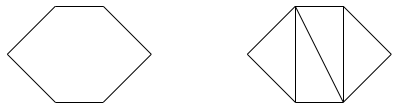
\includegraphics[width=5cm]{hex_tri_cells}
      \caption{Hexagonal cell versus triangle cells}
      \label{fig_hex_vs_tri}
    \end{figure}
  \item[Transition elements and Adaptive Mesh Refinement:] Solvers based on
    arbitrary polyhedral cells can easily handle cells with various number of
    edges. This can be particularly useful for simulations
    with Adaptive Mesh Refinement (AMR) \cite{Jessee1998,Baker2002,Wang2010a}, 
    without having to deal with the implementation of data structures to handle 
    hanging nodes \cite{Solin2008,Bangerth2007,Arnold2000}. On \Cref{fig_amr_cells}, 
    the left cell is a pentagon whereas the two cells on the right are 
    quadrilaterals. A method based on a piecewise linear discretization can
    handle locally adapted meshes without any special treatment or further
    approximation of the coupling between cells.
    \begin{figure}[H]
      \centering
      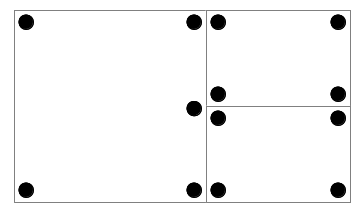
\includegraphics[width=5cm]{amr}
      \caption{AMR mesh}
      \label{fig_amr_cells}
    \end{figure}
\end{description}
Several discretization methods have been developed for arbitrary polygonal
meshes: Palmer's method \cite{Palmer2001}, mimetic finite differences
\cite{Lipnikov2004,Hyman2002,Kuznetsov2004,Brezzi2005},
Wachspress' rationale finite element \cite{Wachspress1975},
CFEM-based DFEM \cite{Warsa2008}, PWLC \cite{Bailey2008a}, PWLD 
\cite{Stone2003,Bailey2008,Bailey2008a}, and PWBLD \cite{Bailey2011}. In this
research, we focus on using PWLD to discretize the diffusion equation. The
PWLD discretization employs discontinuous finite elements and has been used to
discretize the transport equation. Using it to discretize the diffusion
equation is an important step in order to create a Diffusion Synthetic
Acceleration scheme \cite{Adams2002,Wang2010}.
In \Cref{sec_review}, we review different discretizations that can be used on
polygonal cells to discretize the diffusion equation. In \Cref{sec_ip}, we
use the PWLD finite elements to discretize the diffusion
equation. In \Cref{sec_amr}, we introduce the Adaptive Mesh Refinement
technique (AMR). In \Cref{sec_results}, we show some numerical results. We finish
in \Cref{sec_conc} by giving our conclusions.
